\documentclass[a4paper]{article}

\usepackage[utf8]{inputenc}
\usepackage[dutch]{babel}
\usepackage{fancyhdr} %Why the hell does the KU Leuven not have it's own latex header package but the KULAK does?
\usepackage{graphicx}
\usepackage{mathtools}
\usepackage{amssymb}
\usepackage[ruled]{algorithm2e}


\pagestyle{plain}
\title{Numerieke Modellering \& Benadering Practicum 2}
\author{Dennis Debree \and Jonas Bertels}

\begin{document}
\maketitle

\section{Evoluerende kleinste kwadraten problemen}
De eerste stap van het algoritme is de QR-factorizatie van A berekenen. Hierna moet dit niet meer rechtstreeks gebeuren. We beginnen met voor elke k het volgende te doen: We bereken de householder transformatie die moet gebeuren om de matrix $[R_{k}; M_{k}]$ om te zetten naar $[R_{k}; 0]$ waarbij 0 voor een nulmatrix staat met dezelfde dimensies als $M$. Deze householder transformatie $H$ gebruiken we dan om onze nieuwe $Q$ te berekenen door $Q$ eerst te vergroten met eenheidsmatrix van grote dxd op de diagonaal van m tot m+d, en deze dan te vermenigvuldigen met $H$. Hierna kunnen we gemakkelijk het boven-driehoekig stelsel van $Rx = Q*b$ oplossen naar x om zo het antwoord te krijgen.
\section{Rayleigh quotiënt iteratie}
	In deze sectie bespreken we enkele aspecten voor het benaderen van eigen waarden bij symmetrische vierkante matrices.
\subsection{Numerieke stabiliteit}	
	Wanneer de benaderde eigenwaarde $\lambda^{(k-1)}$ dichter in de buurt komt wordt de matrix $A-\lambda^{(k-1)}I$ almaar meer singulier gezien de determinant van deze matrix dichter en dichter bij nul komt.
	In het geval van Rayleigh quotiënt iteration (alsook inverse iteration) vormt dit geen numerieke problemen.
	Dit kunnen we zo inzien:
	Neem een reële symmetrische matrix $A$ met een eigenwaarde veel kleiner in absolute waarde dan de andere.
	Nemen we dan een vector $v$ met componenten in de richtingen van iedere eigenvector bij de eigenwaarden van $A$.
	Los dan $Aw = v$ met een achterwaarts stabiel algoritme op naar $\tilde{w}$.
	Maken we gebruik van de volgende formule (zie p. 95 in 'Numerical Linear Algebra' (L. Trefethen en D. Bau, 1997)):
	\begin{equation}
		\frac{||\delta w||}{||w||}\leq \kappa (A)  \frac{||\delta A||}{||A||}
	\end{equation}
	Waarbij de gelijkheid enkel geldig is indien de berekende vector een veelvoud is van de singuliere vector horende bij de kleinste eigenwaarde van $A$. Gezien de startvector componenten heeft in alle richtingen, is de kans dat we de eigenvector bij de kleinste eigenwaarde benaderen zeer klein, dus zal de relatieve fout veel kleiner zijn dan het slechtste geval.
	\pagebreak
\subsection{Link met kleinste kwadraten probleem}		
	We tonen nu aan dat de oplossing voor het minimalisatie probleem
	\[ \min_{\rho \in \mathbb{R}} ||Ax - \rho x||_2 \]
	overeenkomt met het Rayleigh quotiënt van x.
	
	\vspace{5 mm}
	\noindent Bovenstaande expressie is een kleinste kwadraten probleem waarbij $x\rho \approx Ax$ met $x$ de matrix, $\rho$ de onbekende vector en $Ax$ de rechterhand zijde. Als we met die gegevens de normaalvergelijkingen uitschrijven:
	\begin{align*}
		x^Tx  \rho &= x^TAx \\
		\rho &= \frac{x^TAx}{x^Tx}
	\end{align*}
	Geeft het ons onmiddellijk de formule voor het Rayleigh quotiënt.
\section{Het QR-algoritme}
	We gaan nu over naar een ander algoritme die alle eigenwaarden en bijhorende eigenvectoren van een reële symmetrische matrix $A \in \mathbb{R}^{m \times m}$ kan bepalen, namelijk het QR-algoritme zoals beschreven in algoritme 28.2 uit 'Numerical Linear Algebra' (L. Trefethen en D. Bau, 1997).
\subsection{Enkele eigenschappen}
	Nu tonen we enkele interessante eigenschappen van dit algoritme, hierbij gebruiken we andere theorema's uit hetzelfde boek.
\subsubsection{Behoud van eigenwaarden}
	We tonen nu het behoud van eigenwaarden aan in het algoritme 28.2.
	In het begin van het algoritme wordt de matrix $A$ getridiagonaliseerd. Dit komt neer op een gelijkvormigheidstransformatie met orthogonale matrices dewelke volgens theorema 24.3 de eigenwaarden behoud.
	Ook de deflatie zorgt vanzelfsprekend niet voor verlies van eigenwaarden.
	We tonen nu aan dat het uitrekenen van $A^{k}$ ook de eigenwaarden behoud:
	Gegeven de formules:
	\begin{gather}
		A^{(k-1)} - \mu ^{(k)}I = Q^{(k)}R^{(k)} \\
		A^{(k)} = R^{(k)}Q^{(k)} + \mu ^{(k)}I
	\end{gather}
	Uit (2) bepalen we :
	\begin{equation}
		R^{(k)} = (Q^{(k)})^T(A^{(k-1)}-\mu ^{(k)}I)		
	\end{equation}
	En dan (4) invullen in (3):
	\begin{align}
		A^{(k)} &= (Q^{(k)})^T(A^{(k-1)} - \mu ^{(k)}I)Q^{(k)} + \mu ^{(k)}I\\
		A^{(k)} &= (Q^{(k)})^TA^{(k-1)}Q^{(k)} - \mu ^{(k)}(Q^{(k)})^TQ^{(k)} + \mu ^{(k)}I\\
		A^{(k)} &= (Q^{(k)})^TA^{(k-1)}Q^{(k)}
	\end{align}
	(6) naar (7) gebruikt het feit dat $(Q^{(k)})^TQ^{(k)} = I$.
	Gezien $Q^{(k)}$ een orthogonale matrix is, is dit een gelijkvormigheidstransformatie en dus worden de eigenwaarden behouden.
	
\subsubsection{Behoud van de tridiagonaal vorm}
	We tonen nu aan dat de tridiagonaal vorm behouden wordt in $A^{(k)}$ voor $k = 1,2,\dots$ .
	
	\noindent Gegeven is $A^{(k-1)}$ dat symmetrisch en tridiagonaal is. Een tridiagonaal matrix is automatisch ook bovenhessenberg.
	De gebruikte shifts behouden de tridiagonaal vorm. Zolang $\mu ^{(k)}$ geen exacte eigenwaarde is, kunnen we steeds de QR-factorisatie bepalen. We tonen nu aan dat $A^{(k)} = R^{(k)}Q^{(k)}$ de tridiagonaal vorm bewaart.
	
	\noindent In een QR-factorisatie is $R$ een bovendriehoeks matrix. Gezien de inverse van een bovendriehoeks matrix opnieuw bovendriehoeks is, is $Q^{(k)} = A^{(k-1)}R^{(k)}$ een bovenhessenberg matrix want een bovenhessenberg matrix maal een bovendriehoeks matrix (of omgekeerd) geeft opnieuw een bovenhessenberg matrix.
	
	\noindent Dit geeft ons dan $A^{(k)} = R^{(k)}Q^{(k)}$ wat opnieuw een bovendriehoeks maal bovenhessenberg is, dus is $A^{(k)}$ een bovenhessenberg. Uit (7) weten we dat $A^{(k)}$ via een gelijkvormigheidstransformatie berekend wordt met orthogonale matrices, wat de symmetrie behoud (A symmetrisch, Q orthogonaal):
	\[
		(Q^TAQ)^T = Q^TA^T(Q^T)^T = Q^TA^TQ = Q^TAQ
	\]
	Dus is $A^{(k)}$ symmetrisch en bovenhessenberg dus automatisch tridiagonaal.
\subsection{Een efficiënte implementatie}
Nu we deze handige eigenschappen hebben bewezen, kunnen we ze gebruiken om een efficiënt algoritme te bepalen voor het bepalen van $A(k)$ via (2) en (3).

\noindent We beginnen met het bepalen van de QR-factorisatie: De matrix $A^{(k-1)} - \mu ^{(k)}I$ is een tridiagonaal matrix, deze reduceren kan gemakkelijk door givens-rotaties op ieder subdiagonaal element toe te passen. We houden deze givens-rotaties bij in de matrices $T^{(k)}_1\dots T^{(k)}_m$ zodat we de Q matrix niet expliciet moeten berekenen. Deze is namelijk:
\[
	Q^{(k)} = (T^{(k)}_1)^T(T^{(k)}_2)^T \dots (T^{(k)}_m)^T 
\]
Eens deze bepaald is kunnen we dan $A^{(k)}$ bepalen uit de berekende $R^{(k)}$ en de givens-rotatie matrices (zie ook algoritme 1). 

\noindent Het bepalen van van de matrix  $A^{(k-1)} - \mu ^{(k)}I$ heeft exact $m$ optellingen en $m$ vermenigvuldigingen.
Het bepalen van de $m$ givens-rotaties is iets complexer maar ook een operatie van orde $O(m)$. De hieruit bepaalde $R^{(k)}$ en $T^{(k)}_1\dots T^{(k)}_m$ kunnen dan efficiënt vermenigvuldigd worden gezien er bij de $T^{(k)}_i$ matrices steeds slechts 2 niet diagonaal elementen verschillen van nul. Hieruit volgt dat $R^{(k)}Q^{(k)}$ opnieuw orde $O(m)$ is. Dan is de optelling met $\mu ^{(k)}I$ ook nog van orde $O(m)$ waardoor het volledig algoritme van orde $O(m)$ is.

\begin{algorithm}[H]
	\caption{Iteratie in QR-algoritme}
	\KwIn{$A^{(k-1)}$ tridiagonaal en symmetrisch, $\mu ^{(k)}$}
	\KwOut{$A^{(k)}$}
	\Begin{
		$A^{(k-1)} \leftarrow A^{(k-1)} - \mu ^{(k)}I$\\
		\For{$i = 1 \dots m$}{
			$T_i \leftarrow$ Givens rotatie die element $A^{(k-1)}[i+1,i]$ nul maakt.	\\
			$A^{(k-1)} \leftarrow T_i A^{(k-1)}$ \\
		}
		$A^{(k)} \leftarrow A^{(k-1)}$\\		
		\For{$i = m \dots 1$}{
			$A^{(k)} \leftarrow  A^{(k)}(T_i)^T$\\
		}
		$A^{(k)} \leftarrow$ $A^{(k)} + \mu ^{(k)}I$\\
	}	
\end{algorithm}

\section{Alternatieve eigenwaardenalgoritmen}
	We zagen reeds de Rayleigh quotiënt iteratie en QR-algoritme voor het vinden van eigenwaarden. Er bestaan echter nog andere algoritmes om de eigenwaarden van een symmetrische matrix te bepalen. We bespreken hieronder zo een algoritme.
\subsection{Bisectie-methode}
	De bisectie-methode werkt aan de hand van de interlacing eigenschap van de eigenwaarden van een tridiagonale, symmetrische matrix en de iteratieve methode om nulpunten van een functie te bepalen met de (gelijknamige) bisectie-methode. Hiermee kan je makkelijk de reële eigenwaarden zoeken binnen een bepaald interval.
\subsubsection{Interlacing-eigenschap}
	Neem een symmetrische, tridiagonale matrix $A \in \mathbb{R}^{m\times m} $ die irreduceerbaar is (geen nullen op sub-diagonaal).
	Stel $A^{(1)},\dots ,A^{(m)}$ de boven linkse submatrices van dimensie $1\dots m$.
	Neem nu de eigenwaarden van matrix $A^{(k)}: \lambda _1^{(k)} < \lambda _2^{(k)} < \dots < \lambda _k^{(k)}$
	
	\noindent De interlacing eigenschap zegt dan dat de eigenwaarden van $A^{(k)}$ voldoen aan:
	\begin{equation}
		\lambda _j^{(k)} < \lambda_j^{(k-1)} < \lambda_{j+1}^{(k)}
	\end{equation}
	
	\noindent Hiermee kunnen we makkelijk bepalen hoeveel eigenwaarden er zich bevinden in een bepaald interval $[a,b)$. Uit deze interlacing eigenschap kan je inzien dat je het aantal eigenwaarden die kleiner zijn dan nul kan bepalen door het tellen hoevaak het teken van de determinant veranderd bij als je die voor iedere submatrix achtereenvolgend uitrekent. We weten dat de determinant van een matrix gelijk is aan het product van eigenwaarden van die matrix want:
	
	\begin{align*}
		det(A - xI) &= (\lambda _1 - x)(\lambda _2 - x) \dots (\lambda _m - x)\\
		det(A) &= \lambda _1 \lambda _2 \dots \lambda _m\\ 
	\end{align*}
	Van lijn een naar twee nemen we gewoon $x$ gelijk aan nul.
	Wat hieruit volgt is het gemakkelijkst uit te leggen via een voorbeeld:
	Berekenen we het teken van de determinanten van de submatrices voor matrix $A$ die symmetrisch en tridiagonaal is:
	$ det(A^{(1)}) = 1$, $det(A^{(2)}) = -2$, $det(A^{(3)}) = 4$, $det(A^{(4)}) = 6 $
	Het teken van de eigenwaarde in $A^{(1)}$ is dan uiteraard gelijk aan die van de determinant. Bij $A^{(2)}$ weten we nu dat minstens 1 negatief moet zijn via de formule voor de determinant, en via de interlacing weten we dat er exact 1 positief en 1 negatief moet zijn. Voor $A^{(3)}$ weten we uit de formule voor determinant ofwel geen enkel ofwel 2 eigenwaarden negatief moeten zijn, en via interlacing vinden we dan dat er exact 2 negatief en 1 positief moeten zijn. Voor $A^{(4)}$ moeten er nu 2 of 4 negatief zijn volgens de formula voor de determinant, en via interlacing weten we dat er exact 2 zijn. Dit kan zo verder uitgevoerd worden voor iedere submatrix.
	
	\noindent We illustreren nog eens de interlacing van de eigenwaarden in een simpel voorbeeld, waarbij we de eigenwaarden via de karakteristieke polynoom bepalen zodat we kunnen inzien dat de interlacing eigenschap klopt zonder deze te gebruiken om de eigenwaarden uit te rekenen: 
	Neem de tridiagonale symmetrische matrix A:
	\[ A =
		\begin{bmatrix*}
			1 & 2 & 0 \\
			2 & 3 & 4 \\
			0 & 4 & 5 \\ 
		\end{bmatrix*}
	\]
	Nemen we de eerste submatrix $A^{(1)}$ dan is de eigenwaarde vanzelfsprekend gelijk aan 1.
	Voor de tweede submatrix $A^{(2)}$ kan de karakteristieke polynoom makkelijk bepaald worden: 
	\[
		det(A^{(2)} - \lambda I) = x^2 - 4x - 1 
	\]
	Met nulpunten (dus eigenwaarden) $-0.2361$ en $4.2361$. Dewelke voldoen aan de interlacing eigenschap.
	Voor de matrix $A^{(3)} = A$ is de karakteristieke polynoom nu:
	\[
		det(A - \lambda I) = x^3 -9x^2 + 3x + 21
	\]
	Dus zijn de eigenwaarden $-1.2902$, $1.9520$ en $8.3382$, deze voldoen nu ook aan de interlacing eigenschap.
		
\subsubsection{Pseudoalgoritme}
\begin{verbatim}
function [eigenvalues] = bisection(A,a, b, tol)
if  (signchanges(A,b) - signchanges(A, a))<=0
    eigenvalues = []
elseif (b-a)<tol
    eigenvalues = (a+b)/2
else
    eigenvalues = [bisection(A,a, (a+b)/2, tol), bisection(A,(a+b)/2, b, tol)]


%With help function
function numberOfSignChanges= signchanges(A, x)
    functionk2 = 0
    functionk1 = 1

    numberOfSignChanges= 0
    for k = 1:size(A,1)
        if k > 1
            functionk0 = (A(k, k) - x).* functionk1 - A(k, k-1)^2 .* functionk2         
        else
            functionk0 =(A(k, k) - x)
        if (sign(functionk0) ~= sign(functionk1)) && (sign(functionk0) ~= 0)
            numberOfSignChanges = numberOfSignChanges + 1
        functionk2 = functionk1
        functionk1 = functionk0

\end{verbatim}
\subsubsection{Testproblemen}
Om te kijken of onze functie correct werkte hebben we 2 gevallen berekend:\\
De eerste was een 7x7 matrix die er als volgt uitzag:
\begin{equation}
A =
		\begin{bmatrix*}
			1 & 2 & 0 & 0 & 0 & 0 \\
			2 & 2 & 3 & 0 & 0 & 0 \\
			0 & 3 & 3 & 4 & 0 & 0 \\
			0 & 0 & 4 & 4 & 5 & 0\\
			0 & 0 & 0 & 5 & 5 & 6\\
			0 & 0 & 0 & 0 & 6 & 6\\
			 
		\end{bmatrix*}
\end{equation}
Als we de eigenwaarden die we via ons algoritme vergeleken met de eigenwaarden die we bereikt hebben door de standaard matlab functie eig(A) door de eigenwaarden van elkaar af te trekken en de norm te nemen, dan is het resultaat van onze norm gelijk aan $2.3595*10^{-11}$ bij een tolerantie van $10^{-10}$. We hebben dit testprobleem gekozen omdat het klein genoeg was om de individuele stappen nog te kunnen overlopen en zo te kunnen zien hoe elke eigenwaarde berekent wordt.\\

Daarna gebruikten we een grotere 40x40 matrix die willekeurig werd gegenereerd. Opnieuw was de norm van het verschil tussen de eigenwaarde die matlab berekent en de eigenwaarde die onze functie berekent van de orde $10^{-10}$ (de tolerantie dus). Door een grotere probleemgrootte te kiezen zagen kwamen we nieuwe problemen tegen die ervoor zorgden dat we onze functie opnieuw moesten schrijven.
\subsubsection{Vergelijking met het QR-algoritme}
\begin{figure}
\caption{Vergelijking tijd QR-algoritme en bisectiealgoritme en tolerantie $10^{-13}$}
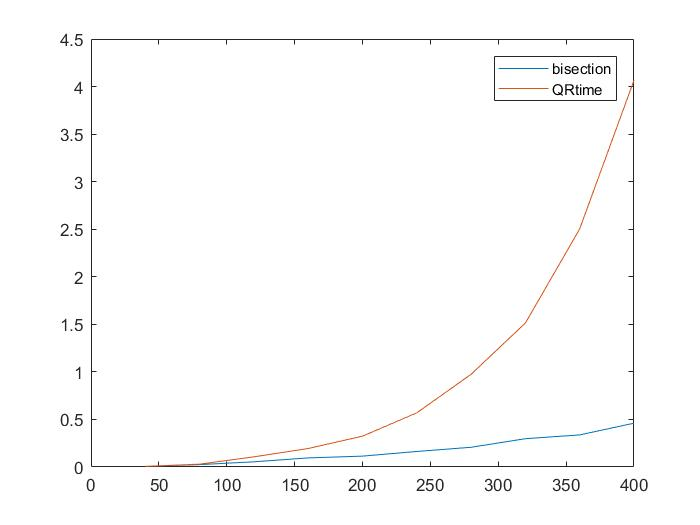
\includegraphics[width=\textwidth, height=0.3\textheight]{QRVSBIPOLAR.JPG}
\end{figure}
We kunnen duidelijk zien dat de hoeveelheid rekenwerk voor een de bisectiemethode lineair stijgt, terwijl de hoeveelheid werk voor de kwadratische methode kwadratisch stijgt afhankelijk van de grootte van de matrix.
\subsubsection{Problemen met de implementatie: recursie van het polynomiaal}
Bij de implementatie van de bisectie-methode in MATLAB kwamen we tegenover enkele interessante problemen te staan. Een eerste was dat het programma exponentieel vertraagde naarmate de matrix groter werd. Rond $n=25$ duurde een volledige oplossing al enkele seconden en $n=30$ duurde zolang dat het niet echt mogelijk was om nog grotere matrices te berekenen. Deze exponentieel stijgende rekentijd klopt natuurlijk niet met de bewering dat de bisectie methode werkt volgens $O(nlog(\epsilon_{mach}))$. \\
Na grondig de code na te kijken bleek dat doordat we de polynoom als een functie bewaren, elke keer dat de functie opgeroepen wordt, 2 andere functies uit de vorige stappen worden opgeroepen om een nieuw resultaat te geven. Omdat hun functiewaarden nergens worden bewaard leidt dit tot $O(2^{n})$ operaties, waardoor het dus onmogelijk wordt om matrices groter dan dimensie 30 uit te rekenen. \\
De oplossing voor dit probleem was de functies te vervangen door lijsten die polynomen voorstellen en deze polynomen dan samen te voegen zodat de berekening van een eigenwaarde voor een gegeven matrix weer $O(nlog(\epsilon_{mach}))$ wordt.
\subsection{De Arnoldi methode}
Als we de resultaten van de Arnoldi methode voor een stijgende hoeveelheid stappen plotten, dan zien we dat de resultaten (in het blauw) steeds dichter bij de cluster van eigenwaarden van de ijle matrix A (in het rood) liggen.
\begin{figure}
\caption{Ritz waarden (in het blauw) en eigenwaarden van A (in het rood) voor 5 stappen}
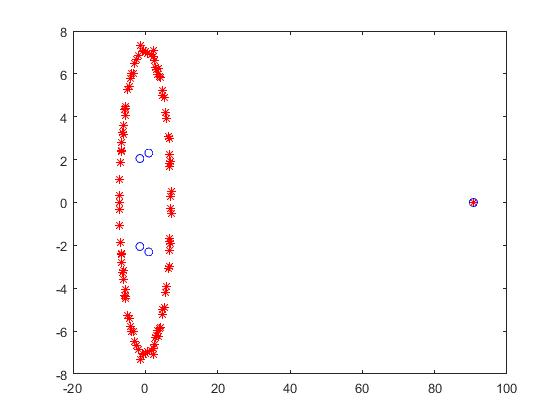
\includegraphics[width=\textwidth, height=0.3\textheight]{RITZ5.JPG}
\end{figure}
\begin{figure}
\caption{Ritz waarden (in het blauw) en eigenwaarden van A (in het rood) voor 10 stappen}
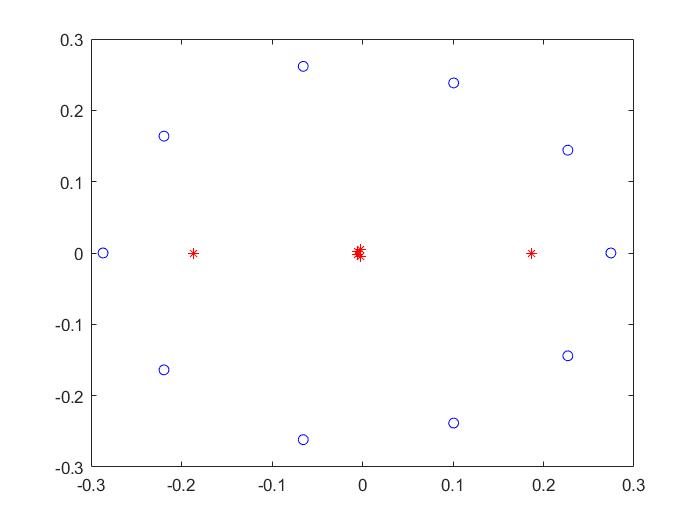
\includegraphics[width=\textwidth, height=0.3\textheight]{RITZ10.JPG}
\end{figure}
\begin{figure}
\caption{Ritz waarden (in het blauw) en eigenwaarden van A (in het rood) voor 20 stappen}
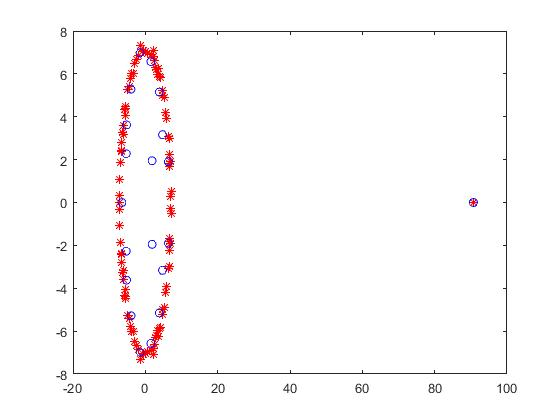
\includegraphics[width=\textwidth, height=0.3\textheight]{RITZ20.JPG}
\end{figure}
\begin{figure}
\caption{Ritz waarden (in het blauw) en eigenwaarden van A (in het rood) voor 100 stappen}
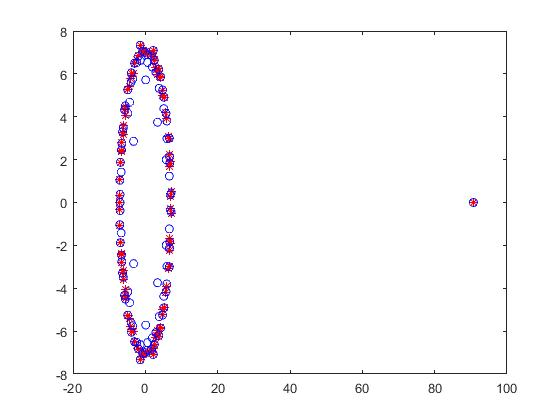
\includegraphics[width=\textwidth, height=0.3\textheight]{RITZ100.JPG}
\end{figure}
\end{document}